% This file was created with tikzplotlib v0.10.1.
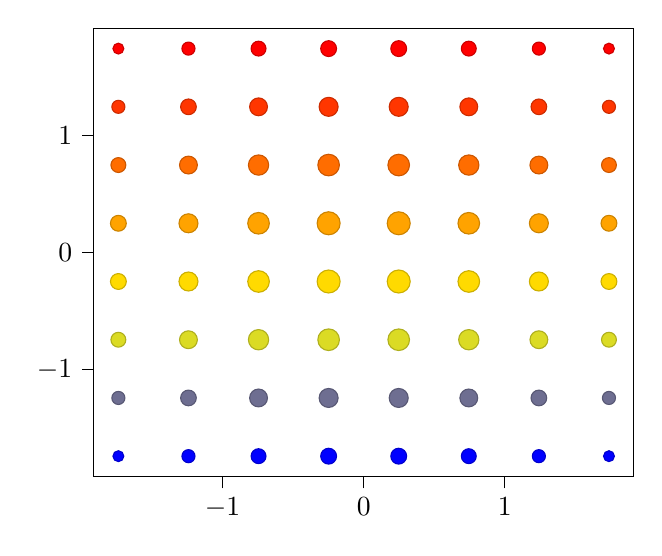
\begin{tikzpicture}

\definecolor{darkgray176}{RGB}{176,176,176}
\definecolor{steelblue31119180}{RGB}{31,119,180}

\begin{axis}[
tick align=outside,
tick pos=left,
x grid style={darkgray176},
xmin=-1.91343339681625, xmax=1.91343339681625,
xtick style={color=black},
y grid style={darkgray176},
ymin=-1.91343339681625, ymax=1.91343339681625,
ytick style={color=black}
]
\addplot [
  draw=steelblue31119180,
  fill=steelblue31119180,
  mark=*,
  only marks,
  scatter,
  scatter/@pre marker code/.append style={/tikz/mark size=\perpointmarksize},
  visualization depends on={\thisrow{sizedata} \as\perpointmarksize}
]
table{%
x  y  sizedata
-1.73948490619659 1.73948490619659 1.9678181
-1.24248933792114 1.73948490619659 2.3599923
-0.745493531227112 1.73948490619659 2.6845918
-0.248497858643532 1.73948490619659 2.859445
0.248497858643532 1.73948490619659 2.859445
0.745493531227112 1.73948490619659 2.6845918
1.24248933792114 1.73948490619659 2.3599923
1.73948490619659 1.73948490619659 1.9678181
-1.73948490619659 1.24248933792114 2.3599923
-1.24248933792114 1.24248933792114 2.8303242
-0.745493531227112 1.24248933792114 3.2196145
-0.248497858643532 1.24248933792114 3.4293149
0.248497858643532 1.24248933792114 3.4293149
0.745493531227112 1.24248933792114 3.2196145
1.24248933792114 1.24248933792114 2.8303242
1.73948490619659 1.24248933792114 2.3599923
-1.73948490619659 0.745493531227112 2.6845918
-1.24248933792114 0.745493531227112 3.2196145
-0.745493531227112 0.745493531227112 3.6624486
-0.248497858643532 0.745493531227112 3.9009922
0.248497858643532 0.745493531227112 3.9009922
0.745493531227112 0.745493531227112 3.6624486
1.24248933792114 0.745493531227112 3.2196145
1.73948490619659 0.745493531227112 2.6845918
-1.73948490619659 0.248497858643532 2.859445
-1.24248933792114 0.248497858643532 3.4293149
-0.745493531227112 0.248497858643532 3.9009922
-0.248497858643532 0.248497858643532 4.155072
0.248497858643532 0.248497858643532 4.155072
0.745493531227112 0.248497858643532 3.9009922
1.24248933792114 0.248497858643532 3.4293149
1.73948490619659 0.248497858643532 2.859445
-1.73948490619659 -0.248497858643532 2.859445
-1.24248933792114 -0.248497858643532 3.4293149
-0.745493531227112 -0.248497858643532 3.9009922
-0.248497858643532 -0.248497858643532 4.155072
0.248497858643532 -0.248497858643532 4.155072
0.745493531227112 -0.248497858643532 3.9009922
1.24248933792114 -0.248497858643532 3.4293149
1.73948490619659 -0.248497858643532 2.859445
-1.73948490619659 -0.745493531227112 2.6845918
-1.24248933792114 -0.745493531227112 3.2196145
-0.745493531227112 -0.745493531227112 3.6624486
-0.248497858643532 -0.745493531227112 3.9009922
0.248497858643532 -0.745493531227112 3.9009922
0.745493531227112 -0.745493531227112 3.6624486
1.24248933792114 -0.745493531227112 3.2196145
1.73948490619659 -0.745493531227112 2.6845918
-1.73948490619659 -1.24248933792114 2.3599923
-1.24248933792114 -1.24248933792114 2.8303242
-0.745493531227112 -1.24248933792114 3.2196145
-0.248497858643532 -1.24248933792114 3.4293149
0.248497858643532 -1.24248933792114 3.4293149
0.745493531227112 -1.24248933792114 3.2196145
1.24248933792114 -1.24248933792114 2.8303242
1.73948490619659 -1.24248933792114 2.3599923
-1.73948490619659 -1.73948490619659 1.9678181
-1.24248933792114 -1.73948490619659 2.3599923
-0.745493531227112 -1.73948490619659 2.6845918
-0.248497858643532 -1.73948490619659 2.859445
0.248497858643532 -1.73948490619659 2.859445
0.745493531227112 -1.73948490619659 2.6845918
1.24248933792114 -1.73948490619659 2.3599923
1.73948490619659 -1.73948490619659 1.9678181
};
\end{axis}

\end{tikzpicture}
